%%%%%%%%%%%%%%%%%%%%%%%%%%%%%%%%%%%%%%%%%%%%%%%%%%%%%%%%%%%%%%%%%%%%%%%%%%
%
% 	Template for seminar reports
%
%%%%%%%%%%%%%%%%%%%%%%%%%%%%%%%%%%%%%%%%%%%%%%%%%%%%%%%%%%%%%%%%%%%%%%%%%%

%%%%%%%%%%%%%%%%%%%%%%%%%%%%%%%%%%%%%%%%%%%%%%%%%%%%%%%%%%%%%%%%%%%%%%%%%%
% 	Include layout and macros
%%%%%%%%%%%%%%%%%%%%%%%%%%%%%%%%%%%%%%%%%%%%%%%%%%%%%%%%%%%%%%%%%%%%%%%%%%
%% This LaTeX template is based on the following example file included in the ieeetran
%% package:
%% bare_conf.tex 
%% V1.2
%% 2002/11/18
%% by Michael Shell
%% mshell@ece.gatech.edu
%% (requires IEEEtran.cls version 1.6b or later) with an IEEE conference paper.


% Note that the a4paper option is mainly intended so that authors in
% countries using A4 can easily print to A4 and see how their papers will
% look in print. Authors are encouraged to use U.S. letter paper when 
% submitting to IEEE. Use the testflow package mentioned above to verify
% correct handling of both paper sizes by the author's LaTeX system.
%
% Also note that the "draftcls" or "draftclsnofoot", not "draft", option
% should be used if it is desired that the figures are to be displayed in
% draft mode.
%
% This paper can be formatted using the peerreviewca
% (instead of conference) mode.
\documentclass[conference, a4paper]{IEEEtran-modified}
% If the IEEEtran.cls has not been installed into the LaTeX system files, 
% manually specify the path to it:
% \documentclass[conference]{../sty/IEEEtran} 

\IEEEoverridecommandlockouts

% some very useful LaTeX packages include:

\usepackage{cite}       % Written by Donald Arseneau
                        % V1.6 and later of IEEEtran pre-defines the format
                        % of the cite.sty package \cite{} output to follow
                        % that of IEEE. Loading the cite package will
                        % result in citation numbers being automatically
                        % sorted and properly "ranged". i.e.,
                        % [1], [9], [2], [7], [5], [6]
                        % (without using cite.sty)
                        % will become:
                        % [1], [2], [5]--[7], [9] (using cite.sty)
                        % cite.sty's \cite will automatically add leading
                        % space, if needed. Use cite.sty's noadjust option
                        % (cite.sty V3.8 and later) if you want to turn this
                        % off. cite.sty is already installed on most LaTeX
                        % systems. The latest version can be obtained at:
                        % http://www.ctan.org/tex-archive/macros/latex/contrib/supported/cite/

%\usepackage{graphicx}  % Written by David Carlisle and Sebastian Rahtz
                        % Required if you want graphics, photos, etc.
                        % graphicx.sty is already installed on most LaTeX
                        % systems. The latest version and documentation can
                        % be obtained at:
                        % http://www.ctan.org/tex-archive/macros/latex/required/graphics/
                        % Another good source of documentation is "Using
                        % Imported Graphics in LaTeX2e" by Keith Reckdahl
                        % which can be found as esplatex.ps and epslatex.pdf
                        % at: http://www.ctan.org/tex-archive/info/
% NOTE: for dual use with latex and pdflatex, instead load graphicx like:
\ifx\pdfoutput\undefined
	\usepackage{graphicx}
\else
	\usepackage[pdftex]{graphicx}
\fi

% However, be warned that pdflatex will require graphics to be in PDF
% (not EPS) format and will preclude the use of PostScript based LaTeX
% packages such as psfrag.sty and pstricks.sty. IEEE conferences typically
% allow PDF graphics (and hence pdfLaTeX). However, IEEE journals do not
% (yet) allow image formats other than EPS or TIFF. Therefore, authors of
% journal papers should use traditional LaTeX with EPS graphics.
%
% The path(s) to the graphics files can also be declared: e.g.,
% \graphicspath{{../eps/}{../ps/}}
% if the graphics files are not located in the same directory as the
% .tex file. This can be done in each branch of the conditional above
% (after graphicx is loaded) to handle the EPS and PDF cases separately.
% In this way, full path information will not have to be specified in
% each \includegraphics command.
%
% Note that, when switching from latex to pdflatex and vice-versa, the new
% compiler will have to be run twice to clear some warnings.
\graphicspath{{figures/}}


%\usepackage{psfrag}    % Written by Craig Barratt, Michael C. Grant,
                        % and David Carlisle
                        % This package allows you to substitute LaTeX
                        % commands for text in imported EPS graphic files.
                        % In this way, LaTeX symbols can be placed into
                        % graphics that have been generated by other
                        % applications. You must use latex->dvips->ps2pdf
                        % workflow (not direct pdf output from pdflatex) if
                        % you wish to use this capability because it works
                        % via some PostScript tricks. Alternatively, the
                        % graphics could be processed as separate files via
                        % psfrag and dvips, then converted to PDF for
                        % inclusion in the main file which uses pdflatex.
                        % Docs are in "The PSfrag System" by Michael C. Grant
                        % and David Carlisle. There is also some information 
                        % about using psfrag in "Using Imported Graphics in
                        % LaTeX2e" by Keith Reckdahl which documents the
                        % graphicx package (see above). The psfrag package
                        % and documentation can be obtained at:
                        % http://www.ctan.org/tex-archive/macros/latex/contrib/supported/psfrag/

%\usepackage{subfigure} % Written by Steven Douglas Cochran
                        % This package makes it easy to put subfigures
                        % in your figures. i.e., "figure 1a and 1b"
                        % Docs are in "Using Imported Graphics in LaTeX2e"
                        % by Keith Reckdahl which also documents the graphicx
                        % package (see above). subfigure.sty is already
                        % installed on most LaTeX systems. The latest version
                        % and documentation can be obtained at:
                        % http://www.ctan.org/tex-archive/macros/latex/contrib/supported/subfigure/

%\usepackage{url}       % Written by Donald Arseneau
                        % Provides better support for handling and breaking
                        % URLs. url.sty is already installed on most LaTeX
                        % systems. The latest version can be obtained at:
                        % http://www.ctan.org/tex-archive/macros/latex/contrib/other/misc/
                        % Read the url.sty source comments for usage information.

%\usepackage{stfloats}  % Written by Sigitas Tolusis
                        % Gives LaTeX2e the ability to do double column
                        % floats at the bottom of the page as well as the top.
                        % (e.g., "\begin{figure*}[!b]" is not normally
                        % possible in LaTeX2e). This is an invasive package
                        % which rewrites many portions of the LaTeX2e output
                        % routines. It may not work with other packages that
                        % modify the LaTeX2e output routine and/or with other
                        % versions of LaTeX. The latest version and
                        % documentation can be obtained at:
                        % http://www.ctan.org/tex-archive/macros/latex/contrib/supported/sttools/
                        % Documentation is contained in the stfloats.sty
                        % comments as well as in the presfull.pdf file.
                        % Do not use the stfloats baselinefloat ability as
                        % IEEE does not allow \baselineskip to stretch.
                        % Authors submitting work to the IEEE should note
                        % that IEEE rarely uses double column equations and
                        % that authors should try to avoid such use.
                        % Do not be tempted to use the cuted.sty or
                        % midfloat.sty package (by the same author) as IEEE
                        % does not format its papers in such ways.

\usepackage{amsmath}    % From the American Mathematical Society
                        % A popular package that provides many helpful commands
                        % for dealing with mathematics. Note that the AMSmath
                        % package sets \interdisplaylinepenalty to 10000 thus
                        % preventing page breaks from occurring within multiline
                        % equations. Use:
\interdisplaylinepenalty=2500
                        % after loading amsmath to restore such page breaks
                        % as IEEEtran.cls normally does. amsmath.sty is already
                        % installed on most LaTeX systems. The latest version
                        % and documentation can be obtained at:
                        % http://www.ctan.org/tex-archive/macros/latex/required/amslatex/math/
%\usepackage[T1]{fontenc}
\usepackage[utf8]{inputenc}
%\usepackage[latin1]{inputenc}   % für Umlaute 
\usepackage{amsfonts}
\usepackage{optidef}
\renewcommand{\keywordname}{Keywords}

% Other popular packages for formatting tables and equations include:

%\usepackage{array}
% Frank Mittelbach's and David Carlisle's array.sty which improves the
% LaTeX2e array and tabular environments to provide better appearances and
% additional user controls. array.sty is already installed on most systems.
% The latest version and documentation can be obtained at:
% http://www.ctan.org/tex-archive/macros/latex/required/tools/

% Mark Wooding's extremely powerful MDW tools, especially mdwmath.sty and
% mdwtab.sty which are used to format equations and tables, respectively.
% The MDWtools set is already installed on most LaTeX systems. The lastest
% version and documentation is available at:
% http://www.ctan.org/tex-archive/macros/latex/contrib/supported/mdwtools/


% V1.6 of IEEEtran contains the IEEEeqnarray family of commands that can
% be used to generate multiline equations as well as matrices, tables, etc.


% Also of notable interest:

% Scott Pakin's eqparbox package for creating (automatically sized) equal
% width boxes. Available:
% http://www.ctan.org/tex-archive/macros/latex/contrib/supported/eqparbox/



% Notes on hyperref:
% IEEEtran.cls attempts to be compliant with the hyperref package, written
% by Heiko Oberdiek and Sebastian Rahtz, which provides hyperlinks within
% a document as well as an index for PDF files (produced via pdflatex).
% However, it is a tad difficult to properly interface LaTeX classes and
% packages with this (necessarily) complex and invasive package. It is
% recommended that hyperref not be used for work that is to be submitted
% to the IEEE. Users who wish to use hyperref *must* ensure that their
% hyperref version is 6.72u or later *and* IEEEtran.cls is version 1.6b 
% or later. The latest version of hyperref can be obtained at:
%
% http://www.ctan.org/tex-archive/macros/latex/contrib/supported/hyperref/
%
% Also, be aware that cite.sty (as of version 3.9, 11/2001) and hyperref.sty
% (as of version 6.72t, 2002/07/25) do not work optimally together.
% To mediate the differences between these two packages, IEEEtran.cls, as
% of v1.6b, predefines a command that fools hyperref into thinking that
% the natbib package is being used - causing it not to modify the existing
% citation commands, and allowing cite.sty to operate as normal. However,
% as a result, citation numbers will not be hyperlinked. Another side effect
% of this approach is that the natbib.sty package will not properly load
% under IEEEtran.cls. However, current versions of natbib are not capable
% of compressing and sorting citation numbers in IEEE's style - so this
% should not be an issue. If, for some strange reason, the user wants to
% load natbib.sty under IEEEtran.cls, the following code must be placed
% before natbib.sty can be loaded:
%
% \makeatletter
% \let\NAT@parse\undefined
% \makeatother
%
% Hyperref should be loaded differently depending on whether pdflatex
% or traditional latex is being used:
%
%\ifx\pdfoutput\undefined
%\usepackage[hypertex]{hyperref}
%\else
%\usepackage[pdftex,hypertexnames=false]{hyperref}
%\fi
%
% Pdflatex produces superior hyperref results and is the recommended
% compiler for such use.

% *** Do not adjust lengths that control margins, column widths, etc. ***
% *** Do not use packages that alter fonts (such as pslatex).         ***
% There should be no need to do such things with IEEEtran.cls V1.6 and later.
%%% This LaTeX template is based on the following example file included in the ieeetran
%% package:
%% bare_conf.tex 
%% V1.2
%% 2002/11/18
%% by Michael Shell
%% mshell@ece.gatech.edu
%% (requires IEEEtran.cls version 1.6b or later) with an IEEE conference paper.


% Note that the a4paper option is mainly intended so that authors in
% countries using A4 can easily print to A4 and see how their papers will
% look in print. Authors are encouraged to use U.S. letter paper when 
% submitting to IEEE. Use the testflow package mentioned above to verify
% correct handling of both paper sizes by the author's LaTeX system.
%
% Also note that the "draftcls" or "draftclsnofoot", not "draft", option
% should be used if it is desired that the figures are to be displayed in
% draft mode.
%
% This paper can be formatted using the peerreviewca
% (instead of conference) mode.
\documentclass[conference, a4paper]{IEEEtran-modified}
% If the IEEEtran.cls has not been installed into the LaTeX system files, 
% manually specify the path to it:
% \documentclass[conference]{../sty/IEEEtran} 

\IEEEoverridecommandlockouts

% some very useful LaTeX packages include:

\usepackage{cite}       % Written by Donald Arseneau
                        % V1.6 and later of IEEEtran pre-defines the format
                        % of the cite.sty package \cite{} output to follow
                        % that of IEEE. Loading the cite package will
                        % result in citation numbers being automatically
                        % sorted and properly "ranged". i.e.,
                        % [1], [9], [2], [7], [5], [6]
                        % (without using cite.sty)
                        % will become:
                        % [1], [2], [5]--[7], [9] (using cite.sty)
                        % cite.sty's \cite will automatically add leading
                        % space, if needed. Use cite.sty's noadjust option
                        % (cite.sty V3.8 and later) if you want to turn this
                        % off. cite.sty is already installed on most LaTeX
                        % systems. The latest version can be obtained at:
                        % http://www.ctan.org/tex-archive/macros/latex/contrib/supported/cite/

%\usepackage{graphicx}  % Written by David Carlisle and Sebastian Rahtz
                        % Required if you want graphics, photos, etc.
                        % graphicx.sty is already installed on most LaTeX
                        % systems. The latest version and documentation can
                        % be obtained at:
                        % http://www.ctan.org/tex-archive/macros/latex/required/graphics/
                        % Another good source of documentation is "Using
                        % Imported Graphics in LaTeX2e" by Keith Reckdahl
                        % which can be found as esplatex.ps and epslatex.pdf
                        % at: http://www.ctan.org/tex-archive/info/
% NOTE: for dual use with latex and pdflatex, instead load graphicx like:
\ifx\pdfoutput\undefined
	\usepackage{graphicx}
\else
	\usepackage[pdftex]{graphicx}
\fi

% However, be warned that pdflatex will require graphics to be in PDF
% (not EPS) format and will preclude the use of PostScript based LaTeX
% packages such as psfrag.sty and pstricks.sty. IEEE conferences typically
% allow PDF graphics (and hence pdfLaTeX). However, IEEE journals do not
% (yet) allow image formats other than EPS or TIFF. Therefore, authors of
% journal papers should use traditional LaTeX with EPS graphics.
%
% The path(s) to the graphics files can also be declared: e.g.,
% \graphicspath{{../eps/}{../ps/}}
% if the graphics files are not located in the same directory as the
% .tex file. This can be done in each branch of the conditional above
% (after graphicx is loaded) to handle the EPS and PDF cases separately.
% In this way, full path information will not have to be specified in
% each \includegraphics command.
%
% Note that, when switching from latex to pdflatex and vice-versa, the new
% compiler will have to be run twice to clear some warnings.
\graphicspath{{figures/}}


%\usepackage{psfrag}    % Written by Craig Barratt, Michael C. Grant,
                        % and David Carlisle
                        % This package allows you to substitute LaTeX
                        % commands for text in imported EPS graphic files.
                        % In this way, LaTeX symbols can be placed into
                        % graphics that have been generated by other
                        % applications. You must use latex->dvips->ps2pdf
                        % workflow (not direct pdf output from pdflatex) if
                        % you wish to use this capability because it works
                        % via some PostScript tricks. Alternatively, the
                        % graphics could be processed as separate files via
                        % psfrag and dvips, then converted to PDF for
                        % inclusion in the main file which uses pdflatex.
                        % Docs are in "The PSfrag System" by Michael C. Grant
                        % and David Carlisle. There is also some information 
                        % about using psfrag in "Using Imported Graphics in
                        % LaTeX2e" by Keith Reckdahl which documents the
                        % graphicx package (see above). The psfrag package
                        % and documentation can be obtained at:
                        % http://www.ctan.org/tex-archive/macros/latex/contrib/supported/psfrag/

%\usepackage{subfigure} % Written by Steven Douglas Cochran
                        % This package makes it easy to put subfigures
                        % in your figures. i.e., "figure 1a and 1b"
                        % Docs are in "Using Imported Graphics in LaTeX2e"
                        % by Keith Reckdahl which also documents the graphicx
                        % package (see above). subfigure.sty is already
                        % installed on most LaTeX systems. The latest version
                        % and documentation can be obtained at:
                        % http://www.ctan.org/tex-archive/macros/latex/contrib/supported/subfigure/

%\usepackage{url}       % Written by Donald Arseneau
                        % Provides better support for handling and breaking
                        % URLs. url.sty is already installed on most LaTeX
                        % systems. The latest version can be obtained at:
                        % http://www.ctan.org/tex-archive/macros/latex/contrib/other/misc/
                        % Read the url.sty source comments for usage information.

%\usepackage{stfloats}  % Written by Sigitas Tolusis
                        % Gives LaTeX2e the ability to do double column
                        % floats at the bottom of the page as well as the top.
                        % (e.g., "\begin{figure*}[!b]" is not normally
                        % possible in LaTeX2e). This is an invasive package
                        % which rewrites many portions of the LaTeX2e output
                        % routines. It may not work with other packages that
                        % modify the LaTeX2e output routine and/or with other
                        % versions of LaTeX. The latest version and
                        % documentation can be obtained at:
                        % http://www.ctan.org/tex-archive/macros/latex/contrib/supported/sttools/
                        % Documentation is contained in the stfloats.sty
                        % comments as well as in the presfull.pdf file.
                        % Do not use the stfloats baselinefloat ability as
                        % IEEE does not allow \baselineskip to stretch.
                        % Authors submitting work to the IEEE should note
                        % that IEEE rarely uses double column equations and
                        % that authors should try to avoid such use.
                        % Do not be tempted to use the cuted.sty or
                        % midfloat.sty package (by the same author) as IEEE
                        % does not format its papers in such ways.

\usepackage{amsmath}    % From the American Mathematical Society
                        % A popular package that provides many helpful commands
                        % for dealing with mathematics. Note that the AMSmath
                        % package sets \interdisplaylinepenalty to 10000 thus
                        % preventing page breaks from occurring within multiline
                        % equations. Use:
\interdisplaylinepenalty=2500
                        % after loading amsmath to restore such page breaks
                        % as IEEEtran.cls normally does. amsmath.sty is already
                        % installed on most LaTeX systems. The latest version
                        % and documentation can be obtained at:
                        % http://www.ctan.org/tex-archive/macros/latex/required/amslatex/math/
%\usepackage[T1]{fontenc}
\usepackage[utf8]{inputenc}
%\usepackage[latin1]{inputenc}   % für Umlaute 
\renewcommand{\keywordname}{Keywords}

% Other popular packages for formatting tables and equations include:

%\usepackage{array}
% Frank Mittelbach's and David Carlisle's array.sty which improves the
% LaTeX2e array and tabular environments to provide better appearances and
% additional user controls. array.sty is already installed on most systems.
% The latest version and documentation can be obtained at:
% http://www.ctan.org/tex-archive/macros/latex/required/tools/

% Mark Wooding's extremely powerful MDW tools, especially mdwmath.sty and
% mdwtab.sty which are used to format equations and tables, respectively.
% The MDWtools set is already installed on most LaTeX systems. The lastest
% version and documentation is available at:
% http://www.ctan.org/tex-archive/macros/latex/contrib/supported/mdwtools/


% V1.6 of IEEEtran contains the IEEEeqnarray family of commands that can
% be used to generate multiline equations as well as matrices, tables, etc.


% Also of notable interest:

% Scott Pakin's eqparbox package for creating (automatically sized) equal
% width boxes. Available:
% http://www.ctan.org/tex-archive/macros/latex/contrib/supported/eqparbox/



% Notes on hyperref:
% IEEEtran.cls attempts to be compliant with the hyperref package, written
% by Heiko Oberdiek and Sebastian Rahtz, which provides hyperlinks within
% a document as well as an index for PDF files (produced via pdflatex).
% However, it is a tad difficult to properly interface LaTeX classes and
% packages with this (necessarily) complex and invasive package. It is
% recommended that hyperref not be used for work that is to be submitted
% to the IEEE. Users who wish to use hyperref *must* ensure that their
% hyperref version is 6.72u or later *and* IEEEtran.cls is version 1.6b 
% or later. The latest version of hyperref can be obtained at:
%
% http://www.ctan.org/tex-archive/macros/latex/contrib/supported/hyperref/
%
% Also, be aware that cite.sty (as of version 3.9, 11/2001) and hyperref.sty
% (as of version 6.72t, 2002/07/25) do not work optimally together.
% To mediate the differences between these two packages, IEEEtran.cls, as
% of v1.6b, predefines a command that fools hyperref into thinking that
% the natbib package is being used - causing it not to modify the existing
% citation commands, and allowing cite.sty to operate as normal. However,
% as a result, citation numbers will not be hyperlinked. Another side effect
% of this approach is that the natbib.sty package will not properly load
% under IEEEtran.cls. However, current versions of natbib are not capable
% of compressing and sorting citation numbers in IEEE's style - so this
% should not be an issue. If, for some strange reason, the user wants to
% load natbib.sty under IEEEtran.cls, the following code must be placed
% before natbib.sty can be loaded:
%
% \makeatletter
% \let\NAT@parse\undefined
% \makeatother
%
% Hyperref should be loaded differently depending on whether pdflatex
% or traditional latex is being used:
%
%\ifx\pdfoutput\undefined
%\usepackage[hypertex]{hyperref}
%\else
%\usepackage[pdftex,hypertexnames=false]{hyperref}
%\fi
%
% Pdflatex produces superior hyperref results and is the recommended
% compiler for such use.

% *** Do not adjust lengths that control margins, column widths, etc. ***
% *** Do not use packages that alter fonts (such as pslatex).         ***
% There should be no need to do such things with IEEEtran.cls V1.6 and later.
%
%%%%%%%%%%%%%%%%%%%%%%%%%%%%%%%%%%%%%%%%%%%%%%%%%%%%%%%%%%%%%%%%%%%%%%%%%%
% 	Anpassung an deutsche Texte
%%%%%%%%%%%%%%%%%%%%%%%%%%%%%%%%%%%%%%%%%%%%%%%%%%%%%%%%%%%%%%%%%%%%%%%%%%

\usepackage{ngerman}
\usepackage[latin1]{inputenc}   % für Umlaute 

%\renewcommand{\abstractname}{Kurzfassung}      % statt Zusammenfassung, wie es ngerman definiert
%\renewcommand{\keywordname}{Schlüsselworte}
%\renewcommand{\figurename}{Abb.}


 %uncomment in case you write in German

%%%%%%%%%%%%%%%%%%%%%%%%%%%%%%%%%%%%%%%%%%%%%%%%%%%%%%%%%%%%%%%%%%%%%%%%%%
% 	Page numbering (not on first page)
%%%%%%%%%%%%%%%%%%%%%%%%%%%%%%%%%%%%%%%%%%%%%%%%%%%%%%%%%%%%%%%%%%%%%%%%%%
\pagestyle{empty}

%%%%%%%%%%%%%%%%%%%%%%%%%%%%%%%%%%%%%%%%%%%%%%%%%%%%%%%%%%%%%%%%%%%%%%%%%%
% 	Correct bad hyphenation here
%%%%%%%%%%%%%%%%%%%%%%%%%%%%%%%%%%%%%%%%%%%%%%%%%%%%%%%%%%%%%%%%%%%%%%%%%%

\hyphenation{}

%%%%%%%%%%%%%%%%%%%%%%%%%%%%%%%%%%%%%%%%%%%%%%%%%%%%%%%%%%%%%%%%%%%%%%%%%%
% 	Begin of the document
%%%%%%%%%%%%%%%%%%%%%%%%%%%%%%%%%%%%%%%%%%%%%%%%%%%%%%%%%%%%%%%%%%%%%%%%%%

\begin{document}

%%%%%%%%%%%%%%%%%%%%%%%%%%%%%%%%%%%%%%%%%%%%%%%%%%%%%%%%%%%%%%%%%%%%%%%%%%
% 	Paper title
%%%%%%%%%%%%%%%%%%%%%%%%%%%%%%%%%%%%%%%%%%%%%%%%%%%%%%%%%%%%%%%%%%%%%%%%%%

\title{Title of the Seminar Paper}

%%%%%%%%%%%%%%%%%%%%%%%%%%%%%%%%%%%%%%%%%%%%%%%%%%%%%%%%%%%%%%%%%%%%%%%%%%
% 	Author names and affiliations 
%		-	multiple columns for up to three different affilitations are separated 
%			by \and
%		- for over three affiliations, refer to ieeetran howto
%%%%%%%%%%%%%%%%%%%%%%%%%%%%%%%%%%%%%%%%%%%%%%%%%%%%%%%%%%%%%%%%%%%%%%%%%%

\author{
\authorblockN{Chengjie Zhou}
\authorblockA{Department of Informatics\\Technische Universität München\\
Email: chengjie.zhou@in.tum.de} 
%\and
%\authorblockN{}
%\authorblockA{}
}

%%%%%%%%%%%%%%%%%%%%%%%%%%%%%%%%%%%%%%%%%%%%%%%%%%%%%%%%%%%%%%%%%%%%%%%%%%
% 	Special paper note (appears between title and authors) 
%%%%%%%%%%%%%%%%%%%%%%%%%%%%%%%%%%%%%%%%%%%%%%%%%%%%%%%%%%%%%%%%%%%%%%%%%%

\specialpapernotice{Seminar Data Mining}

%%%%%%%%%%%%%%%%%%%%%%%%%%%%%%%%%%%%%%%%%%%%%%%%%%%%%%%%%%%%%%%%%%%%%%%%%%
% 	Make title area 
%%%%%%%%%%%%%%%%%%%%%%%%%%%%%%%%%%%%%%%%%%%%%%%%%%%%%%%%%%%%%%%%%%%%%%%%%%

\maketitle

%%%%%%%%%%%%%%%%%%%%%%%%%%%%%%%%%%%%%%%%%%%%%%%%%%%%%%%%%%%%%%%%%%%%%%%%%%
% 	For page number on first page
%%%%%%%%%%%%%%%%%%%%%%%%%%%%%%%%%%%%%%%%%%%%%%%%%%%%%%%%%%%%%%%%%%%%%%%%%%

%\thispagestyle{plain}

%%%%%%%%%%%%%%%%%%%%%%%%%%%%%%%%%%%%%%%%%%%%%%%%%%%%%%%%%%%%%%%%%%%%%%%%%%
% 	Abstract 
%%%%%%%%%%%%%%%%%%%%%%%%%%%%%%%%%%%%%%%%%%%%%%%%%%%%%%%%%%%%%%%%%%%%%%%%%%


\begin{abstract}
This paper provides an overview of the support vector machine (SVM) algorithm
and its applications. SVM is a machine learning algorithm that is widely used
for classification and pattern recognition problems. In this paper, a brief
introduction to the motive of SVM is given. Then, the mathematical background and
definitions of various concepts within the SVM algorithm are stated. Later on,
we discuss the implementation of SVM in various applications, including image
classification, bioinformatics, and so on. Finally, we conclude the paper with
a summary of the advantages and disadvantages of SVM.
\end{abstract}


%%%%%%%%%%%%%%%%%%%%%%%%%%%%%%%%%%%%%%%%%%%%%%%%%%%%%%%%%%%%%%%%%%%%%%%%%%
% 	Keywords 
%%%%%%%%%%%%%%%%%%%%%%%%%%%%%%%%%%%%%%%%%%%%%%%%%%%%%%%%%%%%%%%%%%%%%%%%%%

\begin{keywords}
Data Mining
\end{keywords}


%%%%%%%%%%%%%%%%%%%%%%%%%%%%%%%%%%%%%%%%%%%%%%%%%%%%%%%%%%%%%%%%%%%%%%%%%%
% 	Sections, Subsections,...
%%%%%%%%%%%%%%%%%%%%%%%%%%%%%%%%%%%%%%%%%%%%%%%%%%%%%%%%%%%%%%%%%%%%%%%%%%


\section{Introduction}
One of the most important ascpects of machine learning is classification. Typical algorithms and models
that are used for classification include logistic regression, naive bayes, decision trees and so on. In the early 90s, 
Vladimir Vapnik and his colleagues developed a new algorithm called \emph{Support Vector Machine (SVM)}, which is optimized for classification and regression analysis. In this paper,
we will focus on the main usages of SVM, including the generalization of linear decision boundaries for classification.
We will also discuss the role of kernel in SVM, as well as the implementation, evalution methods, application and many
different aspects of SVM.

In order to thoroughly understand the classification problem, we first need to look at a simple example in one dimension.
Suppose there are two groups of data points that are separately distributed on a one-dimension number line. The classification then
becomes obvious: The threshold that separates both groups simply lies in the middle of the the most outward data points
from both groups. This classification method is called the \emph{maximum margin classifier}, since the margin that separates both
groups is maximized.

\begin{figure}[h]%
    \begin{center}%
        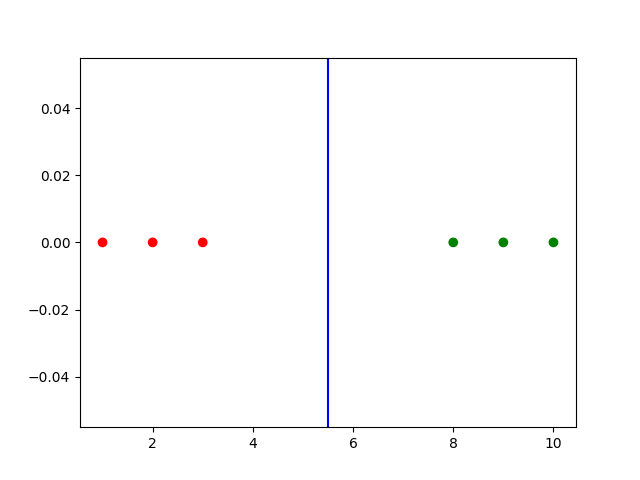
\includegraphics[scale=0.3]{Maximum_Margin_Classifer.png}%
        \caption{Maximum Margin Classfier}\label{fig:}%
    \end{center}%
\end{figure}

Nevertheless, the maximum margin classifier is not always applicable, since the data points are not always idealy distributed
in a separated way. If an outlier happens to appear in the dataset, it would push the threshold to one side, since the data point
is much closer to the other group. This would result in a severe misclassification, since the data that are close to one
group now belongs to the other group because of the shift of the threshold. A solution to this problem is to allow some
misclassification, so that the threshold has higher bias and is less sensitive to outliers and the classifier performs better
when there is new data. This margin that allows some misclassification is called the \emph{soft margin}. The determination of soft margin 
could be tricky, since there are limitless points of thresholds to choose from. One way to find the optimal threshold
is to use Cross Validation. Cross Validation is a method that splits the dataset into several parts. For each repetition, 
one part of the dataset is used for testing and the rest is used for training. After training through all the repetition, the 
average position of the threshold represents the most ideal position of the soft margin. This classifier is called
soft margin classifier, also known as support vector classifier. The name "Support Vector" derives from the fact that
the data points that are closest to the threshold are called support vectors.

\begin{figure}[h]%
    \begin{center}%
        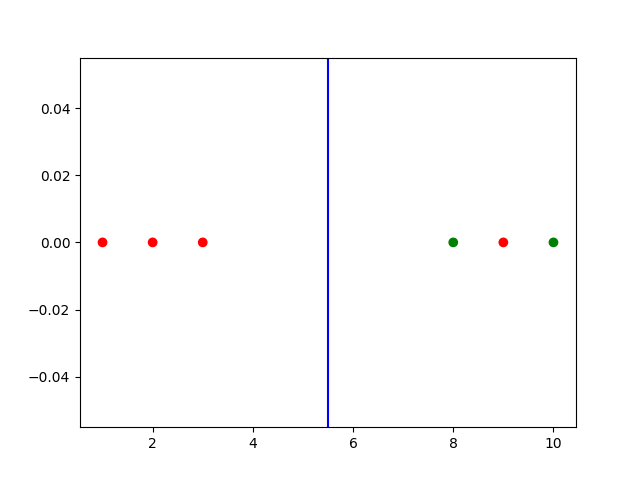
\includegraphics[scale=0.3]{Support_Vector_Classifier.png}%
        \caption{Support Vector Classfier}\label{fig:}%
    \end{center}%
\end{figure}

In reality, chances are that the data is not only one-dimensional. In fact, almost all of the data that we work with
is multi-dimensional. In order to represent the data in a multi-dimensional space, we need to use vectors. In this case,
the idea of hyperplane is introduced. A \emph{hyperplane} is a threshold that separates the data in a multi-dimensional space,
which is formally defined as a flat affine subspace.\cite{R9} The support vector classifier is able to deal with this case as well.
It finds the hyperplane that separates the data in a way that the margin is maximized. The exact algorithms and the
mathematical derivation will be discussed in the next section.

However, the support vector classifier is still not suitable for data that is not linearly separable, even though 
the support vector classifiers allows misclassifications and is less sensitive to outliers.
\begin{figure}[h]%
    \begin{center}%
        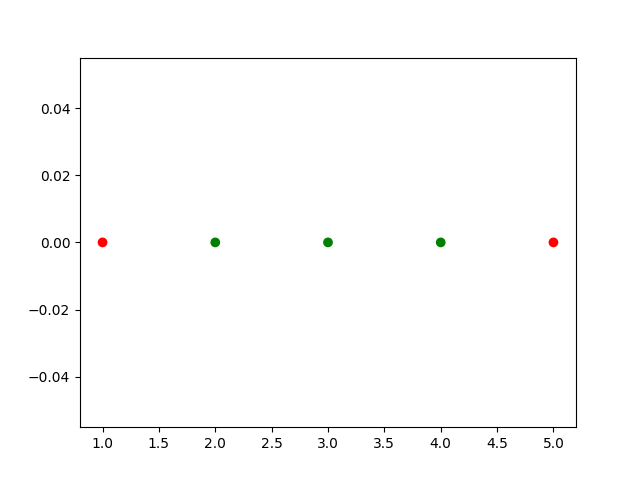
\includegraphics[scale=0.3]{Non_Linearly_Separable_Data.png}%
        \caption{Non Linearly Separable Data}\label{fig:}%
    \end{center}%
\end{figure}

Usually, we use a \emph{kernel} to deal 
with this case, which is a function that maps the data into a higher dimensional space, so that the data becomes linearly
separable. The SVM implements the idea of kernel without transforming the data into a higher dimensional space. This concept is 
called \emph{the kernel trick} and is a crucial part of SVM. This trick allows SVM to cast nonlinear variants to dot products,
enabling easier computation and better performance. \cite{Kernel2}
\begin{figure}[h]%
    \begin{center}%
        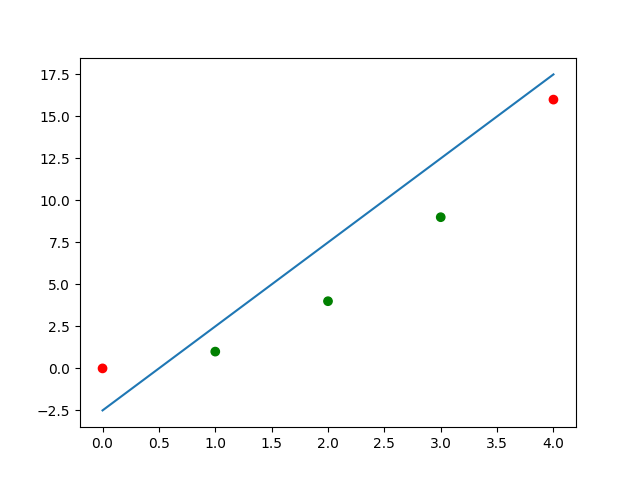
\includegraphics[scale=0.3]{Kernel_Separation.png}%
        \caption{Kernel Transformation}\label{fig:}%
    \end{center}%
\end{figure}

\section{Implementation}
The problem of support vector machine is an optimization problem. The goal is, as mentioned, 
to find the optimal hyperplane that separates the data in a way that the margin is maximized.
Therefore, it is important to first define the hyperplane.

Since the hyperplane is a flat affine subspace of dimension $p$, we can easily define a hyperplane as \cite{R9}: 
\begin{equation}
    \beta_0 + \beta_1X_1 + \beta_2X_2 + ... + \beta_pX_p = 0
\end{equation}

We can then denote $X$ and $\beta$ as vectors \cite{Elements12}: 
\begin{equation}
    \{x \in \mathbb{R}^p: X^T \beta + \beta_0 = 0\}
\end{equation}

With hyperplane being defined, we are now able to observe the problem of separating the hyperplane. 
In other words, we need to construct linear decision
boundaries that attempt to separate the data into two or more classes as precisely as possible. 
The main two mechanics to this problem are Rosenblatt and Optimal.

The \emph{Rosenblatt's perceptron learning algorithm} aims to find the optimal hyperplane in an iterative way. The algorithm minifies
the distance of misclassified points to the decision boundary. The goal of this algorithm is to minimize the following equation
\begin{equation}
    D(\beta, \beta_0) = \sum_{i\in M} -y_i(x_i^T \beta + \beta_0)
\end{equation}
where $M$ is the set of misclassified points and $y_i$ is the class label of $x_i$, being either 1 or -1. Using stochastic gradient
descent, the algorithm updates the coefficients and intercept. 
\begin{equation}
    \partial\frac{D(\beta, \beta_0)}{\partial\beta} = -\sum_{i\in M} y_ix_i
\end{equation}
\begin{equation}
    \partial\frac{D(\beta, \beta_0)}{\partial\beta_0} = -\sum_{i\in M} y_i
\end{equation}
However, the perceptron learning algorithm is not deterministic, since
the result depends on the starting values. Furthermore, the algorithm does not converge if the data is not linearly separable, resulting
in an infinite loop if the case was not detected beforehand. \cite{Elements4}

In 1996, Vapnik proposed the \emph{optimal separating hyperplane} algorithm in order to cope with the problems of the perceptron learning algorithm.
This algorithm is widely implemented as maximum margin classifier.
The goal of the algorithm is to find a hyperplane that maximize the distance to the closet point from either class. [Vapnik, 1996]
The observation of both classes is denoted as $y_i = 1$ and $y_i = -1$. The separating hyperplane then has the following property:

\begin{equation}
    X^T \beta + \beta_0 \geq 1, \text{if}\ y_i = 1
\end{equation}
\begin{equation}
    X^T \beta + \beta_0 \leq -1, \text{if}\ y_i = -1
\end{equation}

To summarize:
\begin{equation}
    y_i(X^T \beta + \beta_0) \geq 1,\ i = 1, ..., n
\end{equation}

To solve this problem, we construct the following optimization problem \cite{R9}:
\begin{equation}
    \begin{aligned}
      & \underset{\textstyle {\beta, \beta_0}}{\text{maximize}} \quad
        M \\
      & \text{subject to} \\
      & ||\beta|| = 1, \\
      & y_i(x_i^T \beta + \beta_0) \geq M,\ i = 1, ..., n
    \end{aligned}
\end{equation}
where $M$ is the margin. Since the margin is $M$ units away from the hyperplane on either side,
the margin is then $2M$ units wide. The constraint $||\beta|| = 1$ can be also left out by replacing
the condition by
\begin{equation}
    \frac{1}{||\beta||}y_i(x_i^T \beta + \beta_0) \geq M
\end{equation}
We arbitrarily set $M = \frac{1}{||\beta||}$. The problem can be then reconstructed as \cite{Elements4}:

\begin{equation}
    \begin{aligned}
      & \underset{\textstyle {\beta, \beta_0}}{\text{maximize}} \quad
        \frac12 ||\beta||^2 \\
      & \text{subject to} \\
      & y_i(x_i^T \beta + \beta_0) \geq 1,\ i = 1, ..., n
    \end{aligned}
\end{equation}

The two constraints of this optimization problem ensures that each observation is on the right side
and has at least a distance of M from the hyperplane. It can be then solved efficiently using
Lagrange functions. The mathematical deduction is beyond the scope of this paper, 
but the result is as follows:
\begin{equation}
    \beta = \sum_{i=1}^n \alpha_i y_i x_i
\end{equation}
\begin{equation}
    0 = \sum_{i=1}^n \alpha_i y_i
\end{equation}
\begin{equation}
    \alpha_i[y_i(x_i^T\beta + \beta_0) - 1] = 0\ \forall i
\end{equation}
where $\alpha$ is a vector of the weights of all the training points as support vectors
under the condition of $\alpha_i \geq 0,\ i = 1, ..., n$. From these three equations, we can
derive the following two properties \cite{Elements4}:
\begin{itemize}
    \item if $\alpha_i > 0$, then $y_i(x_i^T\beta + \beta_0) - 1 = 0$, which is equivalent to
    $y_i(x_i^T\beta + \beta_0) = 0$. This means that the observation is on the margin.
    \item if $y_i(x_i^T\beta + \beta_0) - 1 > 0$, or $y_i(x_i^T\beta + \beta_0) > 1$, then
    $\alpha_i = 0$. This means that the observation is not on the margin.
  \end{itemize}




However, the maximum margin classifier has zero tolerance for misclassification. As mentioned before,
the support vector is designed to be more susceptible to misclassification. With the mathematical knowledge
given above, we can also define the support vector classifier. The hyperplane
is chosen to correctly separate most of the dataset into two classes with the tolerance of a few errors.
Thus, we introduce a slack variable $\epsilon_i$, which allows individual observations to be on the wrong side 
of the margin.
The optimization problem is then defined as\cite{R9}:

\begin{equation}
    \begin{aligned}
      & \underset{\textstyle {\beta, \beta_0, \epsilon, M}}{\text{maximize}} \quad
        M \\
      & \text{subject to} \\
      & ||\beta|| = 1, \\
      & y_i(x_i^T \beta + \beta_0) \geq M(1-\epsilon_i),\ i = 1, ..., n, \\
      & \epsilon_i \geq 0, \ \sum_{i=1}^n \epsilon_i \leq C
    \end{aligned}
\end{equation}

The interpretation of the slack variable helps us to determine whether an observation is on the correct side of the margin.
The $i$th observation is on the correct side of the margin if $\epsilon_i = 0$. Otherwise, 
the $i$th observation is on the wrong side of the margin if $\epsilon_i > 0$ and on the wrong side of the hyperplane
if $\epsilon_i > 1$. The parameter $C$, in this case, is the tuning parameter. It determines the budget of violations
that could happen in this classification problem. The choice of $C$ plays a decisive role in the learning process.
If $C$ is large, then many observations violate the margin, which causes the involvement of many observations in 
determining the hyperplane. On the other hand, smaller $C$s result in a classifier with lower bias but higher variance.
In practice, $C$ is chosen to use cross-validation. 

Based on the optimization problem given above, we can derive the formal definition of SVM. In comparison to 
support vector classifier, the SVM transform the data into a higher dimension space $p'$, so that the data could be
linearly separable. For instance, we transform the features $X_1, X_2, ..., X_p$ into $X_1, X_1^{p'} X_2^{p'}, ..., X_p^{p'}$.
The optimization problem with the transformed data can then be altered to\cite{R9}: 

\begin{equation}
    \begin{aligned}
      & \underset{\textstyle {\beta_0, \beta_{11}, \beta_{12}, ..., \beta_{p(p-1)'}, \beta_{pp'}, \epsilon_1, ..., \epsilon_n, M}}{\text{maximize}} \quad
        M \\
      & \text{subject to} \\
      & y_1(\beta_0 + \sum_{j=1}^p \sum_{k=1}^{p'} \beta_{jk}x_{ij}^k )\geq M (1-\epsilon_i) \\
      & \sum_{i=1}^n\epsilon_i \leq C,\  \epsilon_i \geq 0, \ \sum_{j=1}^p\sum_{k=1}^{p'}\beta_{jk}^2 = 1
    \end{aligned}
\end{equation}

In order to perform the transformation and simplify this problem, we use a kernel function $K(x, x')$. It is defined as \cite{Elements12}:
\begin{equation}
    K(x, x') = \langle h(x), h(x') \rangle
\end{equation}
where $h(x)$ is a transformation function. 
The transformation process leaves us with a lot of freedom, and we are able to freely decide how we should transform the
data. The two popular choices of kernel functions in practical applications are:
\begin{itemize}
    \item dth-Degree Polynomial kernel: $K(x, x') = (1 + \langle x, x' \rangle)^d$
    \item Radial kernel: $K(x, x') = \exp(-\gamma ||x - x'||^2)$
\end{itemize}

First, let us discuss the polynomial kernel. The polynomial kernel transforms each data point into a polynomial
of degree $d$ and fits a support vector classifier into this higher-dimensional space. This 
transformation leads to a flexible decision boundary. 
\begin{equation}
    K(x, x') = (1 + \langle x, x' \rangle)^d = (1 + \sum_{j=1}^px_{ij}x_{i'j})^d
\end{equation}

Another popular choice is the radial kernel. In order to understand the radial kernel, we first need to understand
the following scenario.
If a given test observation $x^*$ is far away from the observation $x_i$,
then the Euclidean distance between the two points will be large.
As the result, the exponential term of the negative value of the Euclidean distance will be close to zero,
which means that the presence of $x^*$ will not have much effect on the transformation.
On the other hand, if $x^*$ is close to $x_i$, then the exponential term will be close to one, which
will exert a strong influence on the transformation. The radial kernel utilizes this property of the
exponential function to emphasize the points that are close to the test observation $x^*$ \cite{R9}.

\begin{equation}
    K(x, x') = \exp(-\gamma ||x - x'||^2) = \exp(-\gamma \sum_{j=1}^p(x_{ij} - x_{i'j})^2)
\end{equation}

The implementation of kernels in SVM saves computational power, since for each pair of data points, we
only need to calculate the transformed value once. Furthermore, the transformative property of the
kernel leads to a flexible and precise boundary. \cite{R9}



\section{Chapter-1}


\subsection{Subchapter}

blabla with three references\cite{ietf-ipfix-protocol,snoeren2001hash,belenky2003ip}

\begin{figure}[h]%
 	\begin{center}%
 		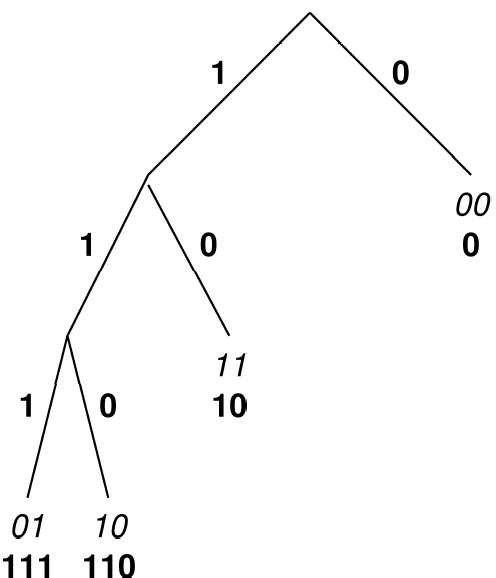
\includegraphics[scale=0.1]{figure1.png}%
 		\caption{Tree}\label{fig:baum}%
 	\end{center}%
\end{figure}

\begin{table}[h]%
 	\begin{center}%
		\caption{Beispieltabelle}\label{tab:example}%
	 	\begin{tabular}{c|c}%
 			Spalte1 & Spalte2\\
 			\hline
 			0 & 1\\
 		\end{tabular}%
 	\end{center}%
\end{table}


%\input{section2}


\section{Conclusion}
In a nutshell, SVM is an algorithm that is capable of solving classification
problems with high accuracy. The main idea of SVM is to find the optimal
hyperplane that separates the data into two classes. In cases where the data
points are not linearly separable, SVM is able to transform 
the dataset in a way that they are linearly separable using kernel functions.
It is a highly automated algorithm that does not require users to deal with
the data distribution properties before applying it. However, its flexibility
also allows users to customize their own kernel functions to transform the data
in a way that suits the real life situation, so that an even better result
could be delivered using these fine-tuning mechanics.

With the properties discussed above, SVM does not really require the users to have deep background
knowledge in the field, since it is highly automated.
The algorithm often delivers high accuracy in binary classification. But it can be modified to deal 
with more complicated problems, such as multi-class classification and
pattern recognition. Its flexibility in usage makes it a popular choice among
researches in many fields. 
Popular applications of SVM include image preprocessing, authentication, natural language
processing, and bioinformatics.
The drawback of SVM is that the interpretation of the
result might be difficult. Nevertheless, we can use data visualization techniques
to help us understand the relationship between the input and the output.


%%%%%%%%%%%%%%%%%%%%%%%%%%%%%%%%%%%%%%%%%%%%%%%%%%%%%%%%%%%%%%%%%%%%%%%%%%
% 	Acknowledgements
%%%%%%%%%%%%%%%%%%%%%%%%%%%%%%%%%%%%%%%%%%%%%%%%%%%%%%%%%%%%%%%%%%%%%%%%%%

%\section*{Acknowledgment}
%\addcontentsline{toc}{section}{Acknowledgment}

%%%%%%%%%%%%%%%%%%%%%%%%%%%%%%%%%%%%%%%%%%%%%%%%%%%%%%%%%%%%%%%%%%%%%%%%%%
% 	References
%%%%%%%%%%%%%%%%%%%%%%%%%%%%%%%%%%%%%%%%%%%%%%%%%%%%%%%%%%%%%%%%%%%%%%%%%%

% trigger a \newpage just before the given reference
% number - used to balance the columns on the last page
% adjust value as needed - may need to be readjusted if
% the document is modified later
%\IEEEtriggeratref{8}
% The "triggered" command can be changed if desired:
%\IEEEtriggercmd{\enlargethispage{-5in}}

% references section
% NOTE: BibTeX documentation can be easily obtained at:
% http://www.ctan.org/tex-archive/biblio/bibtex/contrib/doc/

% can use a bibliography generated by BibTeX as a .bbl file
% standard IEEE bibliography style from:
% http://www.ctan.org/tex-archive/macros/latex/contrib/supported/IEEEtran/bibtex
\bibliographystyle{IEEEtran}
% argument is your BibTeX string definitions and bibliography database(s)
\bibliography{IEEEabrv,references}
%
% <OR> manually copy in the resultant .bbl file
% set second argument of \begin to the number of references
% (used to reserve space for the reference number labels box)
%\begin{thebibliography}{1}
%
%\bibitem{ref:kopka}
%H.~Kopka and P.~W. Daly, \emph{A Guide to {\LaTeX}}, 3rd~ed.\hskip 1em plus
%  0.5em minus 0.4em\relax Harlow, England: Addison-Wesley, 1999.
%
%\end{thebibliography}

%%%%%%%%%%%%%%%%%%%%%%%%%%%%%%%%%%%%%%%%%%%%%%%%%%%%%%%%%%%%%%%%%%%%%%%%%%
% 	End of the document
%%%%%%%%%%%%%%%%%%%%%%%%%%%%%%%%%%%%%%%%%%%%%%%%%%%%%%%%%%%%%%%%%%%%%%%%%%

\end{document}


